\section{Einleitung}
Im Zuge der "`digitalen Revolution"'\footnote{Ähnlich der industriellen Revolution vor 200 Jahren, eine tiefgreifender Wandel von allen gesellschaftlichen Bereichen, wie Politik, Wirtschaft und Kultur. Hervorgerufen durch die Entwicklung von Computern und deren enormen Verbreitung, wird die heutige Zeit auch als "`Zweite Moderne"' bezeichnet} die durch die rasante Entwicklung der Halbleitertechnologien (beschrieben durch das mooresche Gesetz\footnote{Formuliert 1965 von Gordon Moore, der eine Verdopplung der Anzahl von Schaltkreiskomponenten auf einem integrierten Schaltkreis alle 12 bis 24 Monate vorhersagte und damit bis heute Recht bewies.}) ermöglicht wird, übernehmen Computer immer mehr Aufgaben in nahezu allen Bereichen einer modernen Gesellschaft. Neben der industriellen Nutzung finden sich immer mehr Computer in Form mobiler Geräte im Alltag eines jeden Menschen wieder und sie nehmen dabei dem Nutzer viele einfache Aufgaben ab, wie z.B. die Navigation auf einer Straße zu einem Ziel. Durch die steigende Leistungsfähigkeit der Rechensysteme wäre der nächste Schritt auch die höheren Aufgaben auf die Maschinen zu verteilen und somit den Menschen weiter zu entlasten. Eine Aufgabe ist dabei das Führen eines Fahrzeuges ohne menschliches Handeln. Das autonome Fahren ist hierbei keine Fiktion mehr, wie in Filmen wie "`I, Robot"'\cite{iRob}, oder "`Demolition Man"'\cite{DemMan} sugeriert wird, sondern der Prozess ist schon soweit fortgeschritten, dass der autonome Straßenverkehr in naher Zukunft Realität wird. Dafür spricht zum einen, dass schon die ersten autonomen Fahrzeuge des "`EUREKA-PROMETHEUS-Projekts"' \cite{Prom} vor gut 20 Jahren weit mehr als 1758 Km auf öffentlichen Straßen zurückgelegt haben. Und zum anderen, dass in den USA erste autonome Fahrzeuge für den Straßenverkehr zugelassen\cite{Neva} und in Europa zumindest dafür neue Gesetze entworfen werden\cite{Dobri}. So bleibt nur noch die Frage, wann sich der Straßenverkehr auf das autonome Fahren umstellt und wie die Lösung am Ende aussieht.\\ \\
Vor diesem Hintergrund findet der Carolo-Cup in Braunschweig seit nun mehr acht Jahren statt, welcher studentische Teams aller Fachrichtungen und Universitäten in einem Wettbewerb gegeneinander antreten lässt, um das beste Konzept und die beste Umsetzung eines autonomen Fahrzeuges zu präsentieren. Die Otto-von-Guericke-Universität Magdeburg beteiligt sich ebenfalls an diesem Wettbewerb mit dem Projekt "`oTToCAR"'. Die einzelnen Disziplinen sind Einpark,- Spurverfolgungs- und Hindernisszenarien mit Fahrspurwechsel, wofür neben der Hardware- und Software-Entwicklung auch ein Reglungskonzept entwickelt werden muss. Die vorliegenen Arbeit beschäftigt sich mit einer modellbasierten Regelung für alle Szenarien und das dafür verwendete Modell mit der nötigen Parameterschätzung. In einer vorrangegangenen Arbeit \cite{VikAnd} wurde bereits ein Modell entwickelt, deren Parameter jedoch augrund eines fehlenden realen Fahrzeuges nicht bestimmt werden konnten. Die jetzige Arbeit ist zeitlich später einzuordnen, in der ein fertiger Prototyp bereits zur Verfügung stand und die Parameterschätzung vollendet werden konnte. 
\vspace{1cm}
\begin{figure}[H]
\centering
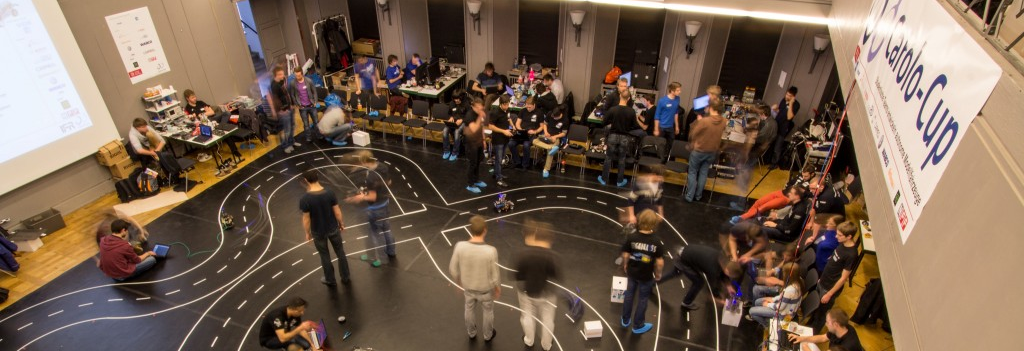
\includegraphics[scale=0.45]{Bilder/Carolo.png}
\caption{Ausschnitt vom Parcours im Carolo-Cup \cite{FotoCaro}}
\end{figure}